\documentclass{beamer}

\usetheme{CambridgeUS}

\renewcommand{\figurename}{}

\usepackage{caption}

\usepackage{hyperref}

\hypersetup{
    colorlinks=true,  
    linkcolor=blue,   
    urlcolor=blue    
}

\captionsetup[figure]{labelsep=none}

\title{Recreating Pac-man}
\subtitle{Bringing classic arcade back}
\author{Krishita Garg, Disha Singla, Yasaswini Devi}
\date{\today}

\begin{document}

\begin{frame}
	\titlepage	
	\begin{figure}
	\centering
    		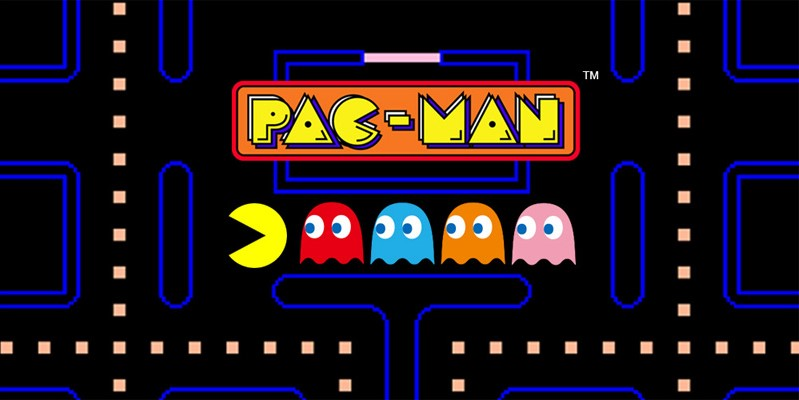
\includegraphics[width=0.25\textwidth]{Pac-man pic}
		\caption{The Original Pac-man}
	\end{figure}
\end{frame}

\begin{frame}{About Pac-man}
        \begin{itemize}
		\item \href{https://pacman.com/en/}{Pac-Man} is a very popular arcade game developed by Toru Itwani for the Namco Company and was first released in Japan on May 22, 1980. 
		\item The main goal of the game is to move the Pac-Man around the maze collecting all the pellets without being eaten by the ghosts. 
		\item Once all of the pellets in the maze have been eaten, the game will begin again on a new maze which will not be the same as the previous map. 
	\end{itemize}
\end{frame}

\begin{frame}{Idea}
	\begin{itemize}
		\item We plan to make a clone of the classic Pac-man game with additional features like 1v1 playing mode and additional themes. 
		\item Our aim is to learn the Pygame framework and graphics tools like GIMP.
	\end{itemize}
\end{frame}

\begin{frame}{Tech Stack}
        \begin{itemize}
                \item Programming Language: Python
		\item Game Framework: Pygame
		\item Graphics: Adobe Photoshop or GIMP
		\item Sound: Audacity for editing, FreeSound.org for sourcing
		\item Version Control: GitLab
		\item Documentation: Markdown (README files)
		\item Communication: Git Issues
        \end{itemize}
\end{frame}

\begin{frame}{Plan Of Action}
        \begin{itemize}
                \item Day 1-2   : Project Setup and Planning
		\item Day 3-5   : Game Mechanics and Basic Functionality
                \item Day 6-9   : UI Design and Theming 
                \item Day 10-11 : Refinement
                \item Day 12    : Sound effects and background music.
		\item Day 13-14 : Finalization, Debugging and Presentation Preparation
        \end{itemize}
\end{frame}


\begin{frame}{Future Scope}
	\begin{itemize}
		\item Enhance multiplayer features.
		\item Integrate AI opponent for single-player mode. 
		\item Both players start as Pac-Man, but one turns into a ghost upon touching a special hidden item and tries to catch the other.
	\end{itemize}
\end{frame}

\begin{frame}
    \centering
    \vfill
    \usebeamerfont{title}\usebeamercolor[fg]{title}\Huge Thank You!
    \vfill
\end{frame}

\end{document}
